\chapter{Kajian Pustaka}

Pada bab ini penulis akan menjelaskan teori yang digunakan selama pengerjaan tugas akhir.

\section{Sudoku}

Sudoku berasal dari kata \textit{Sūji wa dokushin ni kagiru} yang berarti angkanya harus tunggal \cite{SATPy3}. Sebelum sudoku modern berkembang. \textit{Puzzle latin square} terlebih dahulu berkembang yang di repretasikan oleh sebuah matriks berukuran ${n \times n}$ yang memiliki angka ${1 hingga n}$ yang harus diisi oleh pemain. untuk menyelesakain \textit{puzzle }setiap baris dan kolom pada \textit{latin square} harus memiliki nilai angka yang berbeda. \textit{Latin square} pertama kali diciptakan oleh Euler pada tahun 1783 \cite{Unk1}. Sudoku modern sendiri lahir dari  Howard Garns yang dipublikasikan di \textit{Dell Magazines} pada 1979 \cite{SATPy5}. Sudoku dipopulerkan di jepang oleh \textit{Nikoli in the paper Monthly Nikolist} pada April 1984. Sudoku adalah suatu \textit{puzzle} (teka-teki) yang direpresentasikan oleh sebuah matriks (\textit{array}
dua dimensi) berukuran ${n^2 \times n^2}$  yang dibangun dari ${n^2}$ dengan submatriks (atau blok)
yang berukuran ${n \times n}$. Sudoku merupakan \textit{puzzle}
yang biasanya dimainkan oleh satu orang.  Pada
awal permainan, terdapat beberapa sel yang telah terisi yang disebut dengan pemberian
(\textit{givens}). Untuk menyelesaikan permainan ini, seorang pemain harus mengisi setiap sel yang
belum terisi dengan angka di antara 1 sampai
$n^2$ sedemikan sehingga setiap baris, setiap kolom,
dan setiap blok (submatriks berukuran $n \times n$) memuat tepat satu bilangan di antara 1 sampai $n^2$. Biasanya suatu sudoku didesain agar tepat memiliki satu kemungkinan solusi. Hal
ini juga mengakibatkan sudoku dapat diselesaikan hanya dengan mengandalkan penalaran
yang sederhana. Pengisian suatu sel dapat dilakukan dengan meninjau kemungkinan dari
isi sebuah sel. Berikut adalah contoh sudoku $4 \times 4$ dengan tingkat kesulitan mudah serta solusinya:

\begin{figure}[H]
	\begin{centering}
		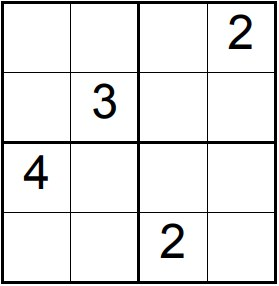
\includegraphics[scale=0.7]{gambar/4x4.jpeg}
		
		\caption{Sudoku dengan \textit{given}.Gambar di ambil dari \cite{SAT423}.}
	\end{centering}
\end{figure}

Pada sel (4,3) terdapat angka 2 sehingga pada blok kiri bawah hanya sel (3,2) saja yang dapat diisi oleh angka 2. Lalu pada sel (1,4) terdapat angka 2 sehingga pada blok kiri atas hanya sel (2,1) saja yang dapat diisi oleh angka 2. Pada sel (2,2) terdapat nilai 3 maka blok kiri bawah hanya dapat mengisi angka 3 pada sel(4,1). Lalu Pada sel (2,2) terdapat nilai 3 maka blok kanan atas hanya dapat mengisi angka 3 pada sel(1,3). Pada blok kiri bawah hanya ada satu sel yang belum terisi maka sel (4,2) diisi dengan angka 1. Pada kolom 1 dan 2 hanya terdapat satu sel yang belum terisi maka kedua sel tersebut diisi dengan angka yang kurang, sel(1,1) angka 1 dan sel (1,2) angka 4. Pada sel(1,3) dan(4,1) terdapat angka 3 sehingga pada blok kanan bawah hanya sel(3,4) yang dapat diisi angka 3. Pada baris 4 hanya satu sel saja yang belum terisi maka sel(4,4) diisi dengan angka 4. Lalu kita dapat mengisi sisanya yaitu sel(2,3) dengan angka 4 lalu sel(2,4) serta (3,3) dengan angka 1.

\begin{figure}[H]
	\begin{centering}
		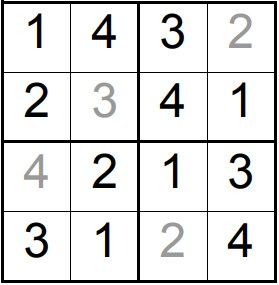
\includegraphics[scale=0.7]{gambar/4x4solved.jpeg}
		
		\caption{Sudoku yang sudah terselesaikan. Gambar di ambil dari \cite{SAT423}.}
	\end{centering}
\end{figure}

	

\section{\textit{Conjunctive Normal Form}(CNF)}

Sebuah formula memiliki bentuk CNF apabila formula tersebut konjungsi dari satu atau lebih klausa dimana klausa adalah disjungsi dari literal \cite{huth2004logic}. Operator yang bisa digunakan dalam CNF adalah $\textit{or}\left(\vee\right)$, $\textit{and}\left(\wedge\right)$, dan, $\textit{not}\left(\neg\right)$. Operator \textit{not} hanya dapat digunakan sebagai bagian dari literal, yang berarti \textit{not} hanya dapat mendahului variabel proposisional.

Berikut adalah contoh formula CNF:
\begin{itemize}
	\item $\left(\left(\ensuremath{x_{1}}\ensuremath{\vee}\ensuremath{x_{2}}\right)\ensuremath{\wedge\neg}\ensuremath{x_{3}}\right)$
	\item $\left(p\vee\neg q\right)$$\wedge$$\left(q\vee\neg r\right)$$\wedge$$\left(r\vee\neg p\right)$
\end{itemize}

Berikut adalah contoh formula yang bukan CNF:
\begin{itemize}
	\item $\neg\left(q\vee p\right)$, karena terdapat \textit{or} didalam \textit{not} 
	\item $p\wedge\left(q\vee\left(r\wedge s\right)\right)$, karena terdapat \textit{and} didalam \textit{or}
	
\end{itemize}

Setiap formula bisa dilakukan kesetaraan agar memiliki bentuk CNF. 

Berikut adalah bentuk CNF dari formula diatas:
\begin{itemize}
	\item $\neg q\wedge p$
	\item $p\wedge\left(q\vee r\right)\wedge\left(q\vee s\right)$
\end{itemize}
\section{\textit{Satisfiability Problem}(SAT)}

Masalah SAT (SAT \textit{problem}) adalah salah satu masalah penting dalam logika komputasional \cite{huth2004logic}. Dalam pengerjaannya SAT berfokus pada membuktikan sebuah klausa \textit{satisfiable} sehingga SAT berfokus pada menemukan sebuah model yang membuat klausa tersebut \textit{satisfiable}. \textit{Satisfiable} yang dimaksud adalah adanya model yang membuat nilai kebenaran dari suatu formula adalah \textit{true}. Jika tidak ditemukan sebuah model yang membuat klausa tersebut \textit{satisfiable} maka klausa tersebut \textit{unsatisfiable}, untuk mengerjakan masalah tersebut dapat diselesaikan menggunakan tabel kebenaran namun hal tersebut kurang efektif, seperti contoh berikut. Tentukan formula berikut $\left(p\vee\neg q\right)$$\wedge$$\left(q\vee\neg r\right)$$\wedge$$\left(r\vee\neg p\right)$ \textit{satisfiable}, pada formula tersebut dibandingkan menggunkan tabel kebenaran kita bisa menggunakan \textit{reasoning}. Dapat kita lihat formula $\left(p\vee\neg q\right)$$\wedge$$\left(q\vee\neg r\right)$$\wedge$$\left(r\vee\neg p\right)$ akan bernilai benar jika ketiga variabel (p, q, dan r) memiliki nilai kebenaran yang sama, sehingga formula tersebut \textit{satisfiable}. Masalah SAT memiliki bentuk CNF serta merupakan masalah NP-complete, hingga saat ini tidak
terdapat algoritma yang efisien untuk memecahkan masalah tersebut. 



\section{Sudoku Sebagai Masalah SAT}
Sudoku memiliki beberapa aturan contohnya untuk sudoku berukuran  $9 \times 9$ yaitu :

\begin{enumerate}
	\item Setiap baris memuat bilangan antara 1 hingga 9.
	\item Setiap kolom memuat bilangan antara 1 hingga 9.
	\item Setiap submatriks atau blok $3 \times 3$
	 memuat bilangan antara 1 hingga 9.
	\item Setiap sel memuat paling banyak satu bilangan antara 1 hingga 9.
\end{enumerate}

Definisi dari $p\left(r,c,n\right)$ adalah sel yang memiliki perpotongan baris $r$ dan kolom $c$ dengan nilai $n$, dengan $1 \leq r,c,n \leq 9$. Sebagai contoh :

\begin{itemize}
	\item $p\left(1,3,2\right)$ berarti sel pada baris 1 dan kolom 3 memuat nilai 2
	\item $p\left(4,2,9\right)$ berarti sel pada baris 4 dan kolom 2 memuat nilai 9
\end{itemize}

Dari aturan-aturan tersebut akan ditranslasikan menjadi bentuk CNF lalu digunakan pada SAT \textit{solver}. Dengan aturan yang telah ditranslasikan dalam CNF sebagai berikut:

\begin{enumerate}
	\item Setiap baris memuat bilangan antara 1 
	hingga 9 : 
	
	$\bigwedge_{r=1}^{9}$$\bigwedge_{n=1}^{9}$$\bigvee_{c=1}^{9}$$p\left(r,c,n\right)$
	
	\item Setiap kolom memuat bilangan antara 1 hingga 9 : 
	
	$\bigwedge_{c=1}^{9}$$\bigwedge_{n=1}^{9}$$\bigvee_{r=1}^{9}$$p\left(r,c,n\right)$
	
	\item Setiap submatriks atau blok $3 \times 3$
	memuat bilangan antara 1 hingga 9 : 
	
	$\bigwedge_{i=0}^{2}$$\bigwedge_{j=0}^{2}$$\bigwedge_{n=1}^{9}$$\bigvee_{r=3i+1}^{3i+3}$$\bigvee_{c=3j+1}^{3j+3}$$p\left(r,c,n\right)$
	
	\item Setiap sel memuat paling banyak satu bilangan antara 1 hingga 9 : 
	
	$\bigwedge_{r=1}^{9}$$\bigwedge_{c=1}^{9}$$\bigwedge_{n=1}^{8}$$\bigwedge_{i=n+1}^{9}$
	$\left(\neg p\left(r,c,n\right)\vee\neg p\left(r,c,i\right)\right)$
	
\end{enumerate}


Pada aturan 1 untuk menyatakan baris $r$ memuat bilangan antara 1 hingga 9, maka dapat ditulis dengan  $\bigvee_{c=1}^{9}$$p\left(r,c,n\right)$. Untuk menyatakan bahwa baris $r$ memuat semua bilangan pada $\left\{1,...,9\right\}$ maka dapat ditulis dengan $\bigwedge_{n=1}^{9}$$\bigvee_{c=1}^{9}$$p\left(r,c,n\right)$. Untuk menyatakan bahwa setiap baris memuat semua bilangan pada $\left\{1,...,9\right\}$ dapat ditulis dengan $\bigwedge_{r=1}^{9}$$\bigwedge_{n=1}^{9}$$\bigvee_{c=1}^{9}$$p\left(r,c,n\right)$

Pada aturan 2  untuk menyatakan kolom $c$ memuat bilangan antara 1 hingga 9, maka dapat ditulis dengan  $\bigvee_{r=1}^{9}$$p\left(r,c,n\right)$
Untuk menyatakan bahwa kolom $c$ memuat semua bilangan pada $\left\{1,...,9\right\}$ maka dapat ditulis dengan $\bigwedge_{n=1}^{9}$$\bigvee_{r=1}^{9}$$p\left(r,c,n\right)$. Untuk menyatakan bahwa setiap kolom memuat semua bilangan pada $\left\{1,...,9\right\}$ dapat ditulis dengan $\bigwedge_{c=1}^{9}$$\bigwedge_{n=1}^{9}$$\bigvee_{r=1}^{9}$$p\left(r,c,n\right)$
 
Pada aturan 3 karena sudoku dengan ukuran $9\times9$ memiliki sel dengan ukuran $3\times3$ maka terdapat 9 blok pada sudoku sehingga :

\begin{figure}[H]
\begin{centering}
	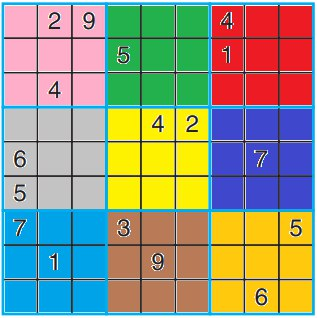
\includegraphics[scale=0.7]{gambar/9x9color.jpeg}
	
	\caption{Gambar sudoku di ambil dari \cite{rosen1995discrete}.}
\end{centering}
\end{figure}

\begin{itemize}
	\item blok pertama(merah muda) akan dimulai pada sel $\left(1,1\right)$ dan di akhiri
	pada sel $\left(3,3\right)$
	\item blok kedua(hijau) akan dimulai pada sel $\left(4,1\right)$ dan di akhiri
	pada sel $\left(6,3\right)$
	\item blok ketiga(merah) akan dimulai pada sel $\left(7,1\right)$ dan di akhiri
	pada sel $\left(9,3\right)$
	\item blok keempat(abu-abu) akan dimulai pada sel $\left(1,4\right)$ dan di akhiri
	pada sel $\left(3,6\right)$
	\item blok kelima(kuning) akan dimulai pada sel $\left(4,4\right)$ dan di akhiri
	pada sel $\left(6,6\right)$
	\item blok keenam(biru) akan dimulai pada sel $\left(7,4\right)$ dan di akhiri
	pada sel $\left(9,6\right)$
	\item blok ketujuh(biru muda) akan dimulai pada sel $\left(1,7\right)$ dan di akhiri
	pada sel $\left(3,9\right)$
	\item blok kedelapan(coklat) akan dimulai pada sel $\left(4,7\right)$ dan di akhiri
	pada sel $\left(6,9\right)$
	\item blok kesembilan(jingga) akan dimulai pada sel $\left(7,7\right)$ dan di akhiri
	pada sel $\left(9,9\right)$
\end{itemize}

Sehingga sebuah blok memuat semua sel $\left(r,c\right)$ dengan $3i+1\leq r\leq3i+3$
dan $3j+1\leq c\leq3j+3$, dengan $0\leq i,j\leq2$. Oleh karena itu aturan 3 dapat ditulis dengan $\bigwedge_{i=0}^{2}$$\bigwedge_{j=0}^{2}$$\bigwedge_{n=1}^{9}$$\bigvee_{r=3i+1}^{3i+3}$$\bigvee_{c=3j+1}^{3j+3}$$p\left(r,c,n\right)$

Pada aturan 4 agar setiap sel memuat angka 1 hingga 9 dapat ditulis dengan $\bigwedge_{r=1}^{9}$$\bigwedge_{c=1}^{9}$$\bigvee_{n=1}^{9}$$p\left(r,c,n\right)$. Lalu agar setiap selnya memiliki paling banyak satu nilai maka nilai pada sel tersebut akan dibandingkan dengan nilai lainnya pada sel yang sama dan jika terdapat dua atau lebih nilai pada sel yang sama maka akan mengeluarkan nilai \textit{false} hal tersebut  dapat ditulis dengan $\bigwedge_{r=1}^{9}$$\bigwedge_{c=1}^{9}$$\bigwedge_{n=1}^{8}$$\bigwedge_{i=n+1}^{9}$
$\left(\neg p\left(r,c,n\right)\vee\neg p\left(r,c,i\right)\right)$.

\section{SAT \textit{Solver}}

SAT \textit{solver} adalah sebuah aplikasi yang dibuat untuk menyelesaikan masalah SAT. Salah satu SAT \textit{solver} yang cepat adalah MiniSat. SAT \textit{solver} sendiri menerima masukan formula dalam bentuk CNF dan mengeluarkan dua buah keluaran yaitu `sat' ditambah sebuah model jika formula \textit{satisfiable}, dan `unsat' jika formula \textit{unsatisfiable}. Format masukan pada SAT \textit{solver} atau yang disebut DIMACS adalah sebagai berikut :

\begin{enumerate}
	\item Pertama baris komentar dapat ditulis dengan: \texttt{c <komentar>}
	\item Lalu banyak variabel dan klausa\texttt{p cnf <banyak-variabel> <banyak-klausa>}
	\item Lalu klausa: 
	
	\begin{itemize}
		\item Setiap variabel di representasikan dengan sebuah integer $\geq1$.
		\item Integer dengan nilai negatif mengartikan negasi literal.
		\item Literal pada sebuah klausa dipisahkan oleh spasi.
		\item Akhir dari klausa ditulis dengan 0
	\end{itemize}
\end{enumerate}

Contoh masukan DIMACS:

Formula : 
$(p\lor q)\land(\neg q\lor r\lor\neg s)\land(s\lor\neg r)$

Ditulis: 

\texttt{c Baris komentar}

\texttt{p cnf 4 3} 

\texttt{1 2 0}

\texttt{-2 3 -4 0}

\texttt{4 -3 0}

\vspace{5mm}


Contoh keluaran SAT \textit{solver}:

Formula: $(p\lor q)\land(\neg q\lor r\lor\neg s)\land(s\lor\neg r)$

\vspace{5mm}

Keluaran:

\texttt{SAT}

\texttt{-1 2 -3 -4 0}

\vspace{5mm}

Untuk penggunaan minisat dapat ditulis dengan:
\texttt{./minisat namaFileMasukan namaFileKeluaran}. Kekurangan pada SAT \textit{solver} adalah solusi \textit{satisfiable} yang dikeluarkan hanyalah satu. Kekurangan ini dapat diatasi dengan memasukkan solusi sebelumnya kedalam salah satu klausa pada masukan DIMACS dalam bentuk negasinya. Proses tersebut akan diulangi sampai keluaran dari SAT \textit{solver} adalah \textit{unsatisfiable}.

\begin{algorithm}
	\caption{Prosedur menemukan semua solusi.}
	\begin{algorithmic}
		\Procedure{Solution}{$in,out,sol$}
		\State \text{Start}
		\State \text{RunSAT(in,out)} 
		\Comment{Menjalankan SAT solver}
		\While{$out[0] \ne 'unsat'$}
		\Comment{Melihat baris pertama pada file out}
		\State \hspace{0.5cm} $sol \leftarrow out[1] $ 
		\Comment{Menambahkan solusi baru} 
		\State \hspace{0.5cm} \textbf{For }$n=0:len(out[1])$\textbf{ do}
		\State \hspace{0.5cm} \hspace{0.5cm} \text{$temp \leftarrow out[1][n] * -1$}
		\Comment{Negasi dari  solusi}
		\State \hspace{0.5cm} \hspace{0.5cm} in $append(temp)$
		\Comment{Menambahkan negasi solusi sebagai klausa baru}
		\State \hspace{0.5cm} \text{RunSAT(in,out)}
		\Comment{Menjalankan SAT solver}
		\EndWhile
		\State \text{End}
		\State \text{Return sol}
		\Comment{Mengeluarkan solusi}
		\EndProcedure
	\end{algorithmic}
	
\end{algorithm}

